\chapter{Geometría sintética}
\section{Planos afines sintéticos}
\begin{definition}[Plano afín]
Un \textbf{plano afín} es un par $\displaystyle \left(\mathcal{P}, \mathcal{R}\right) $ donde $\displaystyle \mathcal{P} $ es un conjunto no vacío cuyos elementos llamamos \textbf{puntos}, y $\displaystyle \mathcal{R} $ es un conjunto de subconjuntos de $\displaystyle \mathcal{P} $ cuyos elementos llamamos \textbf{rectas}, que satisfacen lo siguiente:
\begin{description}
\item[A1.] Sean $\displaystyle P,Q \in \mathcal{P} $ con $\displaystyle P \neq Q $. Existe una única recta $\displaystyle l \in \mathcal{R} $ tal que $\displaystyle P,Q \in l $ (escribimos $\displaystyle l = l\left(PQ\right) $).
\item[A2.] $\displaystyle \forall l \in \mathcal{R}, \forall P \in \mathcal{P} $, $\displaystyle P \not\in l $, existe una única recta $\displaystyle m \in \mathcal{R} $ tal que $\displaystyle P \in m $ y $\displaystyle m \cap l = \emptyset $.
\item[A3.] Toda recta tiene al menos dos puntos y hay al menos dos rectas.
\end{description}
\end{definition}
\begin{observation}
El tercer axioma asegura que se trata de algo dimensional.
\end{observation}
\begin{definition}[Rectas paralelas]
Si $\displaystyle l, m \in \mathcal{R} $ tales que $\displaystyle l \cap m = \emptyset $, diremos que $\displaystyle l $ y $\displaystyle m $ son \textbf{paralelas} y escribimos $\displaystyle l||m $.
\end{definition}
\begin{eg}[Plano cartesiano]
El plano cartesiano $\displaystyle \R^{2} $ es un plano afín. Tenemos que 
\[\mathcal{P  } = \left\{ \left(x_{1}, x_{2}\right) \; : \; x_{1}, x_{2} \in \R\right\}.\]
\[\mathcal{R} : l = \left\{ \left(x_{1}, x_{2}\right) \in \R^{2} \; : \; ax_{1} + bx_{2} = 0, \; a,b,c \in \R, \left(a,b\right) \neq \left(0,0\right)\right\} := \left\{ ax_{1} +bx_{2} = c\right\}  .\]
Vamos a ver que verifica los axiomas. Comprobamos \textbf{A1}. Si tomamos $\displaystyle P = \left(a_{1}, a_{2}\right) $ y $\displaystyle Q = \left(b_{1}, b_{2}\right) $, tenemos que la ecuación de una recta que pasa por $\displaystyle P $ y $\displaystyle Q $ será
\[ \begin{vmatrix} 1 & x_{1} & x_{2} \\ 1 & a_{1} & b_{1} \\ 1 & a_{2} & b_{2} \end{vmatrix} = 0 \iff \left(b_{2}-b_{1}\right)x_{1} + \left(a_{1} - a_{2}\right) x_{2} = a_{1}b_{2}-a_{2}b_{1} .\]
Así, existe una única recta que contiene a $\displaystyle P $ y $\displaystyle Q $. Sabemos que la recta es única porque el sistema
\[
\begin{cases}
ax_{1} + bx_{2} = c \\
a'x_{1} + b'x_{2} = c
\end{cases}
,\]
tiene dos soluciones (porque $\displaystyle P \neq Q $), por lo que tiene infinitas soluciones. Ahora comprobamos el axioma \textbf{A2}. Supongamos que $\displaystyle l = \left\{ ax_{1}+bx_{2} = c\right\}  $, $\displaystyle P = \left(a_{1}, b_{1}\right)\not\in l $, es decir, 
\[a a_{1} + b b_{1} \neq c .\]
Tomamos la recta $\displaystyle m = \left\{ ax_{1} + bx_{2} = a a_{1} + b b_{1}\right\}  $. Tenemos que $\displaystyle P \in m $. Por otro lado, calculamos $\displaystyle m \cap l $:
\[
\begin{cases}
ax_{1} + bx_{2} = c \\
ax_{1} + bx_{2} = a a_{1} + b b_{1}
\end{cases}
.\]
Se trata de un sistema incompatible puesto que $\displaystyle \ran \begin{pmatrix} a & b \\ a & b \end{pmatrix} < \ran \begin{pmatrix} a & b & c \\ a & b &  a a_{1} + b b_{1} \end{pmatrix} $. Así, tenemos que $\displaystyle l \cap m = \emptyset $. La unicidad se deduce de un argumento similar al anterior. En cuanto a \textbf{A3}, tenemos que existe dos rectas $\displaystyle \left\{ x_{1} = 0\right\}  $ y $\displaystyle \left\{ x_{2} = 0\right\}  $, y los puntos $\displaystyle \left(0,\frac{c}{b}\right), \left(\frac{c}{a}, 0\right) \in l = \left\{ ax_{1} + bx_{2} = c\right\}  $.
Si $\displaystyle a = 0 $ o $\displaystyle b = 0 $ tenemos que \textbf{A3} se sigue cumpliendo:
\[ \left(\frac{c}{a}, 0\right), \left(\frac{c}{a}, 1\right) \in \left\{ ax_{1} = c\right\}, \quad \left(0, \frac{c}{b}\right), \left(1, \frac{c}{b}\right) \in \left\{ bx_{2} = c\right\}  .\]
\end{eg}
\begin{observation}
Una recta tiene más de una ecuación asociada. En efecto,
\[l = \left\{ ax_{1} + bx_{2} = c\right\}  = \left\{ \lambda ax_{1} + \lambda bx_{2} = \lambda c\right\}, \; \forall \lambda \in \R / \left\{ 0\right\}  .\]
\end{observation}
\begin{eg}
	Consideremos $\displaystyle \mathcal{P} = \left\{ A, B, C, D\right\}  $ y 
	\[\mathcal{R} = \left\{ \left\{ A,B\right\} , \left\{ A,C\right\} , \left\{ A,D\right\} , \left\{ B, C\right\} , \left\{ B,D\right\} , \left\{ C,D\right\} \right\}  .\]
Tenemos que este plano se corresponde con el gráfico sigiuente:
\begin{center}
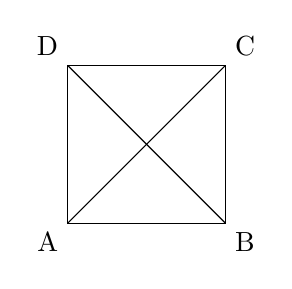
\begin{tikzpicture}[scale=1]
% Define vertices of the square
\coordinate (A) at (0,0);
\coordinate (B) at (2,0);
\coordinate (C) at (2,2);
\coordinate (D) at (0,2);
% Draw the square
\draw (A) -- (B) -- (C) -- (D) -- cycle;
% Draw the diagonals
\draw (A) -- (C);
\draw (B) -- (D);
% Label the vertices
\node[below left] at (A) {A};
\node[below right] at (B) {B};
\node[above right] at (C) {C};
\node[above left] at (D) {D};
\end{tikzpicture}
\end{center}
Se puede ver claramente que \textbf{A1} y \textbf{A2} se cumplen. Es trivial que \textbf{A3} se cumple.	
\end{eg}
\begin{theorem}
Si $\displaystyle \K $ es un cuerpo, entonces $\displaystyle \K^{2} $ es un plano afín con puntos $\displaystyle \K^{2} $ y rectas las ecuaciones lineales.
\end{theorem}
\begin{proof}
Adaptar la demostración del ejemplo del plano cartesiano.
\end{proof}
\begin{eg}
	Consideremos el cuerpo $\displaystyle \mathbb{F}_{2} = \left\{ 0,1\right\}  $ con la suma módulo 2 y el producto también módulo 2.
	Tenemos, por el teorema anterior, el plano afín $\displaystyle \mathbb{F}_{2}^{2} $ de la forma:
	\[\mathbb{F}_{2}^{2} = \left\{ \left(0,0\right), \left(1,0\right), \left(0,1\right), \left(1,1\right)\right\} .\]
	\[\mathcal{R} = \left\{ \left\{ x_{1} = 0\right\}, \left\{ x_{2} = 0\right\}, \left\{ x_{1} = 1\right\}, \left\{ x_{2} = 1\right\}, \left\{ x_{1} + x_{2} = 1\right\} \right\}  .\]
Gráficamente podemos ver que es igual al ejemplo anterior. En este caso, decimos que existe una colineación entre ellos.	
\end{eg}
\subsection{Independencia de los axiomas}
En primer lugar, estudiamos la independencia de \textbf{A3}. Consideremos un ejemplo que satisface \textbf{A1} y \textbf{A2}: $\displaystyle \mathcal{P} = \R $ y $\displaystyle \mathcal{R} = \left\{ l = \R\right\}  $. Así, tenemos que \textbf{A3} es independiente de los otros dos axiomas. \\ \\
Ahora vamos a ver la independencia de \textbf{A2} respecto de \textbf{A1} y \textbf{A3}. Para ello eplearemos el ejemplo del plano de Fano (Gino Fano, 1892):
\[\mathcal{P} = \left\{ A, B, C, D, E, F, G\right\}  .\]
\[\mathcal{R} = \left\{ \left\{ A, B, C\right\}, \left\{ C, D, E\right\}, \left\{ E, F, A\right\}, \left\{ A, G, D\right\}, \left\{ B, G, E\right\}, \left\{ C, G, F\right\} , \left\{ F, B, D\right\} \right\}  .\]
Tenemos que $\displaystyle \left|\mathcal{P}\right| = \left|\mathcal{R}\right| = 7 $. Está claro que se verifica \textbf{A3}, puesto que $\displaystyle \left|\mathcal{R}\right| = 7 $ y $\displaystyle \forall l \in \mathcal{R}, \left|l\right| = 3 $. 
Se puede ver gráficamente que se cumple \textbf{A1} y no se cumple \textbf{A2}, pues cualquier par de rectas se interseca y por tanto no existen rectas paralelas:
% Dibujo
Este es el plano proyectivo más pequeño. \\ \\
Ahora tenemos que estudiar la independencia de \textbf{A1} respecto de \textbf{A2} y \textbf{A3}. Consideremos
\[\mathcal{P}= \left\{ A, B, C, D\right\}  .\]
\[\mathcal{R} = \left\{ \left\{ A, B\right\} , \left\{ C, D\right\} \right\}  .\]
Tenemos que \textbf{A3} se verifica, pues $\displaystyle \left|\mathcal{R}\right| = 2 $ y $\displaystyle \left| \left\{ A,B\right\} \right| = \left| \left\{ C, D\right\} \right| = 2 $. Por otro lado, si $\displaystyle P \not\in \left\{ A,B\right\}  $, tenemos que $\displaystyle P \in \left\{ C,D\right\}  $, por lo que $\displaystyle \left\{ C,D\right\} | | \left\{ A,B\right\}  $. Lo mismo podemos decir si $\displaystyle P \not\in \left\{ C,D\right\}  $. Así, tenemos que se verifica \textbf{A2}. Sin embargo, no se cumple \textbf{A1} porque no existe ninguna recta que contenga a $\displaystyle A $ y $\displaystyle C $.
\subsection{Algunos teoremas}
\begin{lema}[Tricotomía]
Sea $\displaystyle \left(\mathcal{P}, \mathcal{R}\right) $ un plano afín. Sean $\displaystyle l, m \in \mathcal{R} $. Se cumple una y solo una de las siguientes afirmaciones:
\begin{enumerate}
\item $\displaystyle l = m $.
\item $\displaystyle l | | m $.
\item $\displaystyle l \cap m $ es un punto.
\end{enumerate}
\end{lema}
\begin{proof}
Si $\displaystyle l $ no es paralela a $\displaystyle m $, tenemos que $\displaystyle l \cap m \neq \emptyset $. Si $\displaystyle \left|l \cap m\right| = 1 $, tenemos que es un punto y se cumple \textbf{3}. Si $\displaystyle \left|l \cap m\right|\geq 2 $, tenemos que existen $\displaystyle P,Q \in l \cap m $. Por \textbf{A1}, dado que por dos puntos pasa una única recta, debe ser que $\displaystyle m = l $.
\end{proof}
\begin{theorem}[Rectas equipotentes]
Sea $\displaystyle \left(\mathcal{P}, \mathcal{R}\right) $ un plano afín. Todo par de rectas están en biyección.
\end{theorem}
\begin{proof}
Sean $\displaystyle l, m \in \mathcal{R} $.
\begin{description}
\item[Caso 1.] Si $\displaystyle l = m $, es trivial que $\displaystyle l $ y $\displaystyle m $ son equipotentes.
\item[Caso 2.] Supongamos $\displaystyle l \cap m = O $, donde $\displaystyle O \in \mathcal{P} $. Por \textbf{A3}, tenemos que existen $\displaystyle L \in l, M \in m $ tales que $\displaystyle M, L \neq O $. Por \textbf{A1}, existe una única $\displaystyle r \in \mathcal{R} $ tal que $\displaystyle L, M \in r $. Si $\displaystyle P \in l/ \left\{ L\right\}  $, tenemos que existe una única $\displaystyle r_{p} | | r $ tal que $\displaystyle P \in r_{p} $. 
\begin{center}
	\begin{tikzpicture}
% Coordinates
\coordinate (O) at (0,1);
\coordinate (L) at (-2,-1); % on l
\coordinate (M) at (2,-1);  % on m
\coordinate (P) at (-1,0); % between L and O on l

% Lines l and m through O
\draw (-2.5,-1.5) -- (0.5,1.5) node[right] {$l$};
\draw (2.5,-1.5) -- (-0.5,1.5) node[left] {$m$};

% Line r (horizontal) through L and M
\draw (L) -- (M) node[midway, above] {$r$};

% Dashed line through P parallel to r (horizontal)
%\draw[dashed] (P) -- ($(P)+(1,0)$);
%\draw[dashed] (P) -- ($(P)+(-1,0)$);
\draw[dashed] (-1.3,0) -- (1.3,0) node[above] {$r_p$};

% Points
\fill (O) circle (0.7pt) node[above] {$O$};
\fill (L) circle (0.7pt) node[left] {$L$};
\fill (M) circle (0.7pt) node[right] {$M$};
\fill (P) circle (0.7pt) node[left] {$P$};

% Axes for reference
\draw[->, thin] (-1.2,0) -- (1.2,0) node[right] {$x$};
\draw[->, thin] (0,-0.2) -- (0,2.5) node[above] {$y$};
\end{tikzpicture}
	\end{center}

	Podemos hacer un par de observaciones:
	\begin{description}
		\item[Observación 1.] Vamos a ver que $\displaystyle \forall P \in l/ \left\{ L\right\}  $ tenemos que $\displaystyle P \not\in r$, queremos ver que $\displaystyle r _{p} $ existe. Si $\displaystyle P \in l \cap r $, tenemos que $\displaystyle L, P \in l \cap r $, por lo que $\displaystyle l = r $, por lo que $\displaystyle M \in l $ y $\displaystyle O,M \in l  $ y $\displaystyle l = m $, que es una contradicción. Por tanto, podemos afirmar que $\displaystyle \forall P \in l $, $\displaystyle P \neq L $, $\displaystyle \exists r_{p} $ recta paralela a $\displaystyle r $ y $\displaystyle P \in r_{p} $.
		\item[Observación 2.] Tenemos que ver que $\displaystyle r_{p} \cap m $ es un punto. Si $\displaystyle r_{p} | | m $, como $\displaystyle r_{p} | | r $, $\displaystyle M \in m $ y $\displaystyle M \in r $, se tiene que $\displaystyle m = r $, por lo que $\displaystyle L \in r = m $ y $\displaystyle O \in m $, por lo que $\displaystyle m = l $, lo que es una contradicción. Por otro lado, si $\displaystyle r_{p} = m $, $\displaystyle P \in l $ y $\displaystyle P \in r_{p} = m $ y $\displaystyle O \in m,l $, por lo que $\displaystyle m = l $, que es una contradicción. Por tanto, debe ser que $\displaystyle r_{p}\cap m $ es un punto.
	\end{description}
	De esta manera, podemos definir la función
	\[
	\begin{split}
		f : l / \left\{ L\right\} & \to m / \left\{ M\right\} \\
		P & \to r_{p} \cap m.
	\end{split}
	\]
	Para ver que $\displaystyle f $ es biyectiva, vamos a ver que existe su inversa. En efecto, tenemos que $\displaystyle \forall Q \in m / \left\{ M\right\}  $, $\displaystyle Q \not\in r $ y $\displaystyle r_{Q}\cap l $ es un punto. Así, tenemos una función
	\[
	\begin{split}
		g : m/ \left\{ M\right\} & \to l / \left\{ L\right\} \\
		Q & \to r_{Q} \cap l.
	\end{split}
	\]
Para ver que $\displaystyle g = f^{-1} $ tenemos que ver que $\displaystyle g\circ f = id $ y que $\displaystyle f\circ g = id $:
\[
\begin{split}
	\left(g \circ f\right)\left(P\right) & = g\left(f\left(P\right)\right) = g\left(r_{p} \cap m\right) .
\end{split}
\]
Tenemos que $\displaystyle r_{f\left(P\right)} = r _{r_{p} \cap m} | | r $ y $\displaystyle r_{f\left(P\right)} $ pasa por $\displaystyle r_{p} \cap m $. Pero $\displaystyle r_{p} | | r $ y $\displaystyle r_{p} $ pasa por $\displaystyle r_{p} \cap m $. Por \textbf{A2}, tenemos que $\displaystyle r_{f\left(P\right)} = r_{p} $. Así, tenemos que
\[g\left(r_{p} \cap m\right) = r_{f\left(P\right)} \cap l = r_{p} \cap l = P .\]
\item[Caso 3.] Si $\displaystyle m | | l $ y $\displaystyle M \in m $, $\displaystyle L \in l $, tenemos que existe una recta $\displaystyle r $ tal que $\displaystyle M, L \in r $. Así, tenemos que $\displaystyle r \cap m $ y $\displaystyle r \cap l $ es un punto y por lo aplicado en el caso anterior, tenemos que existe una biyección entre $\displaystyle r $ y $\displaystyle m $ y entre $\displaystyle r $ y $\displaystyle l $.
	% Dibujo 3
\end{description}
\end{proof}
\begin{lema}
Sea $\displaystyle \left(\mathcal{P}, \mathcal{R}\right) $ un plano afín. Ponemos $\displaystyle l \sim m $, $\displaystyle l, m \in \mathcal{R} $, si $\displaystyle  l = m  $ o $\displaystyle l | | m $. Entonces, $\displaystyle \sim $ es una relación de equivalencia.
\end{lema}
\begin{proof}
\begin{description}
\item[(i)] Está claro que si $\displaystyle l \in \mathcal{R} $ se tiene que $\displaystyle l = l $, por lo que se cumple la propiedad reflexiva. 
\item[(ii)] Sean $\displaystyle l,m \in \mathcal{R} $. Si $\displaystyle l = m $ es trivial que se cumple la propiedad simétrica. Si $\displaystyle l \sim m $ y $\displaystyle l | | m $, tenemos que $\displaystyle l \cap m = m \cap l = \emptyset $, por lo que $\displaystyle m \sim l $. Así, hemos verificado la propiedad simétrica.
\item[(iii)] Sean $\displaystyle l,m,r \in \mathcal{R} $ con $\displaystyle l \sim m $ y $\displaystyle m \sim r $. Hay que valorar varios casos:
	\begin{description}
	\item[Caso 1.] Si $\displaystyle l = m $ y $\displaystyle m = r $, está claro que $\displaystyle l = r $ y, por tanto, $\displaystyle l \sim r $.
	\item[Caso 2.] Si $\displaystyle l = m $ y $\displaystyle m | | r $, está claro que $\displaystyle l \cap r = m \cap r = \emptyset $, por lo que $\displaystyle l \sim r $.
	\item[Caso 3.] Si $\displaystyle l | | m $ y $\displaystyle m = r $, tenemos que $\displaystyle l \cap r = l \cap m = \emptyset $, por lo que $\displaystyle l \sim r $.
	\item[Caso 4.] Si $\displaystyle l | | m  $ y $\displaystyle m | | r $, está claro que $\displaystyle l \cap m = m \cap r = \emptyset $, por lo que $\displaystyle l \sim r $.
	\end{description}
	Así, queda demostrada la propiedad transitiva.
\end{description}
\end{proof}

\begin{definition}[Haz de rectas]
Un \textbf{haz de rectas paralelas} es una clase de equivalencia de $\displaystyle \sim $. Entonces, $\displaystyle \mathcal{H} \subset \mathcal{R}  $ es un \textbf{haz} si y solo si $\displaystyle \exists l \in \mathcal{R} $ tal que 
\[\mathcal{H} = [l]_{\sim} = \left\{ m \; | \; m = l \; \text{o} \; m | | l\right\}  .\]
\end{definition}
\begin{prop}
Sea $\displaystyle \mathcal{H} $ un haz y $\displaystyle l \in \mathcal{R} $ con $\displaystyle l \not\in \mathcal{H} $, entonces $\displaystyle f: \mathcal{H} \to l : m \to l \cap m $ es una biyección.
\end{prop}
\begin{proof}
\begin{description}
\item[(i)] Primero vamos a ver que la función está bien definida. Como $\displaystyle l \not\in \mathcal{H} $, $\displaystyle \forall m \in \mathcal{H} $ tenemos que $\displaystyle l  $ no es paralelo a $\displaystyle m $ y $\displaystyle l \neq m $. Por el lema de la tricotomía, debe ser que $\displaystyle l \cap m $ es un punto. Así, la función está bien definida.
\item[(ii)] Veamos que la función es inyectiva. Consideremos $\displaystyle m_{1}, m_{2} \in \mathcal{H} $ tales que $\displaystyle m_{1} \cap l = m_{2} \cap l \neq \emptyset $, por lo que $\displaystyle m_{1} \cap m_{2} \neq \emptyset $. Dado que $\displaystyle m_{1}, m_{2} \in \mathcal{H} $, tenemos que $\displaystyle m_{1} \sim m_{2} $ y como $\displaystyle m_{1} $ no es paralela a $\displaystyle m_{2} $, debe ser que $\displaystyle m_{1} = m_{2}$.
\item[(iii)] Comprobemos que la aplicación es sobreyectiva. Supongamos que $\displaystyle P \in l $, $\displaystyle  m \in \mathcal{H} $. Si $\displaystyle P \in m $, tenemos que $\displaystyle m \cap l = P $, por lo que hemos ganado. Si $\displaystyle  P \not\in m $, por \textbf{A2} tenemos que existe $\displaystyle m_{1} \in \mathcal{H} $ (es decir, paralela a $\displaystyle m $) tal que $\displaystyle P \in m_{1} $, por lo que $\displaystyle P = m_{1} \cap l $.
\end{description}
\end{proof}
\begin{prop}
Si $\displaystyle \mathcal{H}_{1} $ y $\displaystyle \mathcal{H}_{2} $ son dos haces distintos, tenemos que $\displaystyle \forall P \in \mathcal{P} $, $\displaystyle \exists! l \in \mathcal{H}_{1}, \exists! m \in \mathcal{H}_{2} $ tales que  $\displaystyle P = l \cap m $. En particular, la aplicación $\displaystyle f: \mathcal{H}_{1} \times \mathcal{H}_{2} \to \mathcal{P} : \left(l, m\right) \to l \cap m$ es una biyección.
\end{prop}
\begin{proof}
Supongamos que 
\[\mathcal{H}_{1} = \left[l\right] _{\sim} = \left\{ l' \; | \; l' = l \; \text{o} \; l' | | l\right\}  .\]
\[\mathcal{H}_{2} = \left[m\right] _{\sim} = \left\{ m' \; | \; m' = m \; \text{o} \; m' | | m\right\} .\]
Tenemos que dado que $\displaystyle \mathcal{H}_{1} \neq \mathcal{H}_{2} $, tenemos que $\displaystyle l \neq m $ y $\displaystyle l $ no es paralelo a $\displaystyle m $, por lo que $\displaystyle l \cap m $ es un punto. Así, hemos visto que la aplicación está bien definida.\\
Sea $\displaystyle P \in \mathcal{P} $:
\begin{description}
\item[Caso 1.] Si $\displaystyle P \in l $ hemos terminado.
\item[Caso 2.] Si $\displaystyle P \not\in l $, por \textbf{A2} existe una única recta $\displaystyle l' \in \mathcal{H}_{1} $ tal que $\displaystyle P \in l' $.
\end{description}
En ambos casos, tenemos que $\displaystyle \exists! l_{1} \in \mathcal{H}_{1} $ tal que $\displaystyle P \in l_{1} $. Así, simétricamente existe una única $\displaystyle m_{1} \in \mathcal{H}_{2} $ tal que $\displaystyle P \in m_{1} $. 
\end{proof}
\subsection{Planos afines finitos}
\begin{definition}
Un plano afín tiene \textbf{orden} $\displaystyle n $ si todas sus rectas tienen $\displaystyle n $ elementos.
\end{definition}
\begin{observation}
La definición tiene sentido dado que todas las rectas tienen el mismo número de puntos.
\end{observation}
\begin{theorem}
Sea $\displaystyle \left(\mathcal{P}, \mathcal{R}\right) $ una plano afín de orden $\displaystyle n $. 
\begin{description}
\item[(i)] Cada haz de rectas tiene $\displaystyle n $ elementos.
\item[(ii)] $\displaystyle \left|\mathcal{P}\right| = n^{2} $.
\item[(iii)] Cada punto está en $\displaystyle n + 1 $ rectas.
\item[(iv)] Hay $\displaystyle n + 1 $ haces de rectas.
\item[(v)] Hay $\displaystyle n\left(n+1\right) $ rectas.
\end{description}
\end{theorem}
\begin{proof}
Sea $\displaystyle \left(\mathcal{P}, \mathcal{R}\right) $ un plano afín de orden $\displaystyle n $.
\begin{description}
\item[(i)] Sea $\displaystyle \mathcal{H} $ un haz de rectas. Por \textbf{A3}, existe $\displaystyle l_{1}, l_{2} \in \mathcal{R} $ con $\displaystyle l_{1} \neq l_{2} $. Si existe $\displaystyle l \not\in \mathcal{H} $ hemos ganado. Si $\displaystyle l_{1}, l_{2} \in \mathcal{H} $, sea $\displaystyle P \in l_{1} $ y $\displaystyle Q\in l_{2} $, tenemos que $\displaystyle l\left(P,Q\right) \not\in \mathcal{H} $ por lo que existe $\displaystyle l \not\in \mathcal{H} $. Por una proposición anterior, tenemos que existe una biyección entre $\displaystyle \mathcal{H}  $ y $\displaystyle l $, por lo que $\displaystyle \left|\mathcal{H}\right| = \left|l\right| = n $.
\item[(ii)] Por el argumento del apartado anterior, existen $\displaystyle l, m \in \mathcal{R} $ con $\displaystyle l \neq m $ y que no son paralelas entre sí, tales que $\displaystyle \mathcal{H}_{1} = \left[l\right]_{\sim}  $ y $\displaystyle \mathcal{H}_{2} = \left[m\right]_{\sim}  $. Por la proposición anterior, tenemos que $\displaystyle \left|\mathcal{H}_{1} \times \mathcal{H}_{2}\right| = \left|\mathcal{P}\right| $. Por la primera propiedad, nos queda que $\displaystyle \left|\mathcal{P}\right| = \left|\mathcal{H}_{1}\right| \cdot \left|\mathcal{H}_{2}\right| = n^{2} $.
\item[(iii)] Sea $\displaystyle P \in \mathcal{P} $. Por \textbf{A3} es fácil deducir que existe una recta $\displaystyle l \in \mathcal{R} $ tal que $\displaystyle P \not\in l $. Tenemos que $\displaystyle l = \left\{ A_{1}, \ldots, A_{n}\right\}  $, por lo que $\displaystyle P \in l\left(P, A_{1}\right), \ldots, l\left(P, A_{n}\right) $. 
	Por \textbf{A2}, existe una única paralela $\displaystyle m $ a $\displaystyle l $ tal que $\displaystyle P \in m $, por lo que $\displaystyle P $ está en $\displaystyle n + 1 $ rectas. En efecto, todas las rectas anteriores son distintas porque de no serlo tendríamos que 
	\[l\left(P, A_{i}\right) = l\left(P, A_{j}\right) \Rightarrow l\left(P, A_{i}\right) = l\left(A_{i}, A_{j}\right) = l \Rightarrow P \in l .\]
	Si $\displaystyle r \in \mathcal{R} $ tal que $\displaystyle P \in r $, por \textbf{A2} se sigue que o $\displaystyle r \cap l = \emptyset $, por lo que $\displaystyle r = m $; o $\displaystyle r \cap l = A_{i} $, por lo que $\displaystyle r = l\left(P, A_{i}\right) $.
\item[(iv)] Por \textbf{(iii)}, dado $\displaystyle P \in \mathcal{P} $, existen $\displaystyle l_{1}, \ldots, l_{n+1} \in \mathcal{R} $ con $\displaystyle P \in l_{i} $, $\displaystyle \forall i = 1, \ldots, n +1$. Como $\displaystyle l_{i} \cap l_{j} = P $, tenemos que $\displaystyle \left[l_{i}\right]_{\sim} \neq \left[l_{j}\right]_{\sim}  $ si $\displaystyle i \neq j $. Por tanto hay al menos $\displaystyle n + 1 $ haces. Sea $\displaystyle r \in \mathcal{R} $, 
	\begin{itemize}
	\item Si $\displaystyle P \in r $, tenemos que $\displaystyle r = l_{i} $ para algún $\displaystyle 1 \leq i \leq n +1 $.
	\item Si $\displaystyle P \not\in r $, por \textbf{A2} tenemos que existe una única $\displaystyle l_{i} $ tal que $\displaystyle r | | l_{i} $, por lo que $\displaystyle P \in l_{i} $.
	\end{itemize}
	En ambos casos tenemos que $\displaystyle r \in \left[l_{i}\right] _{\sim} $ para algún $\displaystyle i $.
\item[(v)] Los haces son distintos dos a dos, por ser una relación de equivalencia. Por tanto, 
	\[ \left|\mathcal{R}\right| = \left|\bigcup_{i = 1}^{n+1}\mathcal{H}_{i}\right| = \sum^{n + 1}_{ i = 1} \left|\mathcal{H}_{i}\right| = \sum^{n+1}_{i = 1}n = n\left(n+1\right) .\]
\end{description}
\end{proof}
\begin{observation}
Para todo primo $\displaystyle p $ y todo $\displaystyle k \geq 1 $, existe un cuerpo $\displaystyle \K $ con $\displaystyle p^{k} $ elementos. Entonces, $\displaystyle \forall p $ primo y $\displaystyle \forall k \geq 1 $, existe un plano afín de orden $\displaystyle p ^{k} $, porque $\displaystyle \K^{2} $ es un plano afín.
\end{observation}
\section{Planos proyectivos sintéticos}
\begin{definition}[Plano proyectivo]
Un \textbf{plano proyectivo} es un par $\displaystyle \left(\overline{\mathcal{P}}, \overline{\mathcal{R}}\right) $ donde $\displaystyle \overline{\mathcal{P}} $ es un conjunto no vacío cuyos elementos se llaman \textbf{puntos} y $\displaystyle \overline{\mathcal{R}} $ es un conjunto de subconjuntos de $\displaystyle \overline{\mathcal{P}} $ cuyos elementos se llaman \textbf{rectas}. Se cumplen los axiomas:
\begin{description}
\item[P1.] Para cada par de puntos distintos existe una única recta que los contiene.
\item[P2.] Todo par de rectas tiene intersección no vacía.
\item[P3.] Toda recta tiene al menos tres puntos y hay al menos dos rectas.
\end{description}
\end{definition}
En primer lugar, vamos a comprobar la consistencia de la definición, es decir, que hemos definido algo que existe.
\begin{eg}[Plano de Fano]
Consideremos los conjuntos 
\[\overline{\mathcal{P}} = \left\{ A, B, C, D, E, F, G\right\}  .\]
\[\overline{\mathcal{R}} = \left\{ \left\{ A,B,C\right\} , \left\{ C, D, E\right\} , \left\{ E, F, A\right\} , \left\{ B, G, F\right\} , \left\{ A, G, D\right\}, \left\{ F, G, C\right\}, \left\{ F, D, B\right\} \right\}  .\]
\begin{center}
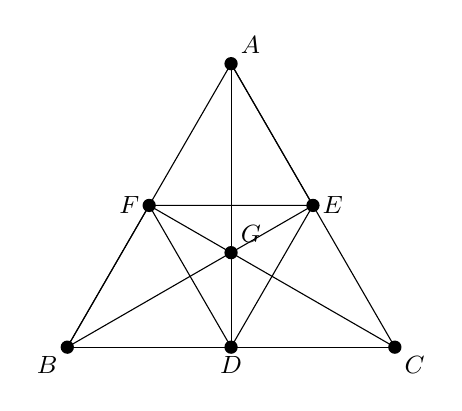
\begin{tikzpicture}[scale=2, every node/.style={font=\small}]

% --- Definir coordenadas explícitas ---
\coordinate (A) at (0,1.2);
\coordinate (B) at (-1.04,-0.6);
\coordinate (C) at (1.04,-0.6);

\coordinate (F) at (-0.52,0.3); % aprox. punto medio de AB
\coordinate (D) at (0,-0.6);    % aprox. punto medio de BC
\coordinate (E) at (0.52,0.3);  % aprox. punto medio de CA

\coordinate (G) at (0,0);       % centro

% --- Dibujar las rectas del plano de Fano ---
% 1) Lado AB
\draw (A) -- (B);
% 2) Lado BC
\draw (B) -- (C);
% 3) Lado CA
\draw (C) -- (A);
% 4) Triángulo interior DEF
\draw (D) -- (E) -- (F) -- cycle;
% 5) Medianas
\draw (A) -- (E);
\draw (B) -- (F);
\draw (C) -- (D);
\draw (A) -- (D);
\draw (F) -- (C);
\draw (B) -- (E);

% --- Dibujar puntos ---
\foreach \pt in {A,B,C,D,E,F,G} {
  \fill (\pt) circle (1.2pt);
}

% --- Nombres ---
\node[above right] at (A) {$A$};
\node[below left]  at (B) {$B$};
\node[below right] at (C) {$C$};

\node[below] at (D) {$D$};
\node[right] at (E) {$E$};
\node[left]  at (F) {$F$};

\node[above right] at (G) {$G$};

\end{tikzpicture}
\end{center}
Es fácil comprobar que se trata de un plano proyectivo.
\end{eg}
\begin{observation}
Este es el plano proyectivo más pequeño, es decir, que tiene menos puntos.
\end{observation}
\subsection{Independencia de los axiomas}
\begin{itemize}
	\item Comprobamos la independencia de \textbf{P3} respecto de \textbf{P2} y \textbf{P1}. Consideremos el ejemplo $\displaystyle \overline{\mathcal{P}}= \R $ y $\displaystyle \overline{\mathcal{R}} = \left\{ \R\right\} $. Está claro que se cumplen \textbf{P1} y \textbf{P2} pero no se cumple \textbf{P3}.
	\item Comprobamos la independencia de \textbf{P2} respecto de \textbf{P1} y \textbf{P3}. Consideremos como ejemplo el plano afín $\displaystyle \R^{2} $. Tenemos que \textbf{A1} es igual que \textbf{P1}, hay rectas paralelas, por lo que \textbf{P2} no se cumple y está claro que se cumple \textbf{P3} puesto que $\displaystyle \left|\overline{\mathcal{R}}\right| = \infty, \forall \overline{l} \in \overline{\mathcal{R}} , \left|\overline{l}\right|=\infty$.
	\item Comprobamos la independencia de \textbf{P1} respecto de \textbf{P2} y \textbf{P3}. Consideremos por ejemplo:
		\[\overline{\mathcal{P}} = \left\{ A, B, C, D, E\right\}  .\]
		\[\overline{\mathcal{R}} = \left\{ \left\{ A, B, C\right\}, \left\{ C, D, E\right\} \right\}  .\]
Claramente se cumple \textbf{P3} y se cumple \textbf{P2} porque hay dos rectas y las dos se intersecan. No se cumple \textbf{P1} puesto que no existe $\displaystyle \overline{l} \in \overline{\mathcal{R}} $ tal que $\displaystyle A , D \in \overline{l} $.
\end{itemize}
\subsection{Algunos teoremas}
\begin{theorem}
Sea $\displaystyle \K $ es un cuerpo y $\displaystyle \K^{3} $ un espacio vectorial. Sean 
\[\overline{\mathcal{P}} = \left\{ U \subset \K^{3} \; : \; U \in \mathcal{L}\left(\K^{3}\right), \dim _{\K}U = 1\right\}  .\]
\[\overline{\mathcal{R}} = \left\{ W \subset \K^{3} \; : \; W \in \mathcal{L}\left(\K^{3}\right), \dim _{\K} W = 2\right\}  .\]
Entonces, $\displaystyle \left(\overline{\mathcal{P}}, \overline{\mathcal{R}}\right) $ es un plano proyectivo 
\footnote{La definición de $\displaystyle \overline{\mathcal{R}} $ es más bien el conjunto de los conjuntos de rectas que son contenidas por un plano, así se puede hacer una correspondencia biyectiva entre $\displaystyle \overline{\mathcal{R}} $ y la descripción que le hemos dado. Así, decimos que un punto $\displaystyle \overline{P} \in \overline{\mathcal{P}} $ está en una recta $\displaystyle \overline{l} \in \overline{\mathcal{R}} $ si $\displaystyle \overline{P} $ está contenido en el plano que caracteriza a $\displaystyle \overline{l} $.} .
\end{theorem}
\begin{proof}
\begin{description}
	\item[(i)] Vamos a ver que se cumple \textbf{P1}. Si $\displaystyle P,Q \in \overline{\mathcal{P}} $ con $\displaystyle P \neq Q $, existen $\displaystyle \vec{v}_{1}, \vec{v}_{2} \in \K^{3} $ linealmente independientes tales que $\displaystyle P = L\left( \left\{ \vec{v}_{1}\right\} \right) $ y $\displaystyle Q = L\left( \left\{ \vec{v}_{2}\right\} \right) $.
		Así, existe $\displaystyle r \in \overline{\mathcal{R}} $ tal que $\displaystyle r = L\left( \left\{ \vec{v}_{1}, \vec{v}_{2}\right\} \right) $ que cumple que $\displaystyle P, Q \subset r $. En concreto, tenemos que $\displaystyle r = P \oplus Q $. \\
	 Sea $\displaystyle r_{2} \in \overline{\mathcal{R}} $ tales que $\displaystyle P,Q \subset r_{2} $, entonces tenemos que $\displaystyle P \oplus Q \subset r_{2} $ y $\displaystyle \dim\left(P\oplus Q\right) = \dim r_{2} $, por lo que $\displaystyle r_{2} = r $.
\item[(ii)] Vamos a ver que se cumple \textbf{P2}. Sean $\displaystyle l,m \in \overline{\mathcal{R}} $, tenemos que 
	\[\underbrace{\dim\left(l \cap m\right)} _{\leq 3} = \underbrace{\dim l}_{2} + \underbrace{\dim m}_{2} - \underbrace{\dim\left(l \cap m\right)}_{\geq 1} .\]
	Por tanto, $\displaystyle \dim\left(l \cap m\right) \geq 1 $, por lo que $\displaystyle l \cap m \neq \emptyset $.
\item[(iii)] Vamos a ver que se cumple \textbf{P3}. Sea $\displaystyle \K^{3} = L\left( \left\{ \vec{u}_{1}, \vec{u}_{2}, \vec{u}_{3}\right\} \right) $, sean $\displaystyle r_{1} = L\left( \left\{ \vec{v}_{1}, \vec{v}_{2}\right\} \right) $ y $\displaystyle r_{2} = L\left( \left\{ \vec{u}_{1}, \vec{u}_{3}\right\} \right) $ dos rectas. Así, hemos visto que hay al menos dos rectas.
	Ahora, dada una recta $\displaystyle r = L(\left\{ \vec{v}_{1}, \vec{v}_{2}\right\} ) $ tenemos que $\displaystyle P_{1} = L\left( \left\{ \vec{v}_{1}\right\} \right) $, $\displaystyle P_{2} = L\left( \left\{ \vec{v}_{2}\right\} \right) $ y $\displaystyle P_{3} = L\left( \left\{ \vec{v}_{1} + \vec{v}_{2}\right\} \right) $ son puntos de la recta. Así, hemos visto que cada recta tiene al menos tres puntos.
\end{description}
\end{proof}
\begin{definition}
	Sea $\displaystyle \K $ un cuerpo. Al plano proyectivo construido en el teorema anterior lo llamamos \textbf{proyectivizado de} $\displaystyle \K^{3} $ y lo denotamos por $\displaystyle \mathbb{P}\left(\K^{3}\right) $.
\end{definition}
\begin{notation}
	Dado $\displaystyle \left(a_{0}, a_{1}, a_{2}\right) \in \K^{3} $ denotamos por $\displaystyle \left[a_{0}: a_{1}: a_{2}\right]  $ al punto $\displaystyle L\left( \left\{ \left(a_{0}, a_{1}, a_{2}\right)\right\} \right) $. Observamos que 
	\[ \left[a_{0} : a_{1} : a_{2}\right] = \left[b_{0} : b_{1} : b_{2}\right] \iff L\left( \left\{ \left(a_{0}, a_{1}, a_{2}\right)\right\} \right) = L\left( \left\{ \left(b_{0}, b_{1}, b_{2}\right)\right\} \right).\]
	Esto es cierto si y solo si existe $\displaystyle \lambda \in \K/ \left\{ 0\right\}  $ tal que $\displaystyle \left(a_{0}, a_{1}, a_{2}\right) = \lambda \left(b_{0}, b_{1}, b_{2}\right) $. Así, tenemos que esta notación está bien definida salvo proporcionalidad. Así, tenemos que los puntos de $\displaystyle \mathbb{P}\left(\K^{3}\right) $ son 
	\[ \left\{ \left[a_{0} : a_{1} : a_{2}\right] \; : \; \left(a_{0}, a_{1}, a_{2}\right) \in \K^{3} / \left\{ 0\right\} \right\}  .\]
	Por otro lado, si $\displaystyle u \in \K^{3} $ tal que $\displaystyle \dim\left(u\right) = 2 $, podemos describir $\displaystyle u $ con una ecuación implícita homogénea:
	\[u = \left\{ \left(x_{0}, x_{1}, x_{2}\right) \; : \; ax_{0} + bx_{1} + c_{2} = 0\right\}  .\]
	Decimos que $\displaystyle \overline{l} $ es la recta $\displaystyle ax_{0} + bx_{1} + cx_{2} = 0 $. Tenemos que si $\displaystyle \left(u_{0}, u_{1}, u_{2}\right) \in \overline{l} $, entonces $\displaystyle \left(\lambda u_{0}, \lambda u_{1}, \lambda u_{2}\right) \in \overline{l} $. En efecto, 
	\[au_{0} + bu_{1} + cu_{2} = 0 \Rightarrow a\lambda u_{0} + b\lambda u_{1} + c\lambda u_{2} = 0.\]
	Así hemos visto que $\displaystyle \left[u_{0} : u_{1} : u_{2}\right] \in \overline{l} $ si y solo si $\displaystyle au_{0} + bu_{1} + cu_{2} = 0 $, por lo que $\displaystyle \left[u_{0} : u_{1} : u_{2}\right] \in \overline{l} $ está bien definido. Definimos $\displaystyle \mathbb{P}\left(\K^{3}\right) $ de la siguiente forma,
	\[\overline{\mathcal{P}} = \left\{ \left[a_{0} : a_{1} : a_{2}\right]  \; : \; a_{i} \in \K/ \left\{ 0\right\} \right\}  .\]
	\[\overline{\mathcal{R}} = \left\{ ax_{0} + bx_{1} + cx_{2} = 0\right\} \footnote{Claramente $\displaystyle a $, $\displaystyle b $ y $\displaystyle c $ no son 0 simultáneamente.}  .\]
	Podemos observar que si $\displaystyle P = [a_{0} : a_{1} : a_{2}] $ y $\displaystyle Q = [b_{0}:b_{1}:b_{2}] $ con $\displaystyle P \neq Q $, se cumple que
	\[\overline{l}\left(P,Q\right) = \left\{ \begin{vmatrix} x_{0} & x_{1} & x_{2} \\ a_{0} & a_{1} & a_{2} \\ b_{0} & b_{1} & b_{2} \end{vmatrix} = 0\right\}   .\]
	
\end{notation}
\subsection{Construcción de planos proyectivos desde planos afines}
Sea $\displaystyle \left(\mathcal{P}, \mathcal{R}\right) $ un plano afín. 
\begin{itemize}
\item Para cada haz de rectas $\displaystyle \mathcal{H} $ creamos un punto $\displaystyle P_{\mathcal{H}} $ \footnote{Este punto es distinto para cada haz de rectas.}.
\item Cogemos $\displaystyle \overline{\mathcal{P}} = \mathcal{P} \cup \left\{ P_{\mathcal{H}} \; : \; \mathcal{H} \; \text{haz de rectas}\right\}  $.
\item Dado $\displaystyle l \in \mathcal{R} $ con $\displaystyle l \in \mathcal{H} $, ponemos $\displaystyle \overline{l} = l \cup \left\{ P_{\mathcal{H}}\right\}  $.
\item Ponemos $\displaystyle \overline{l}_{\infty} = \left\{ P_{\mathcal{H}} \; : \; \mathcal{H} \; \text{haz de rectas}\right\}  $.
\item Tomamos $\displaystyle \overline{\mathcal{R}} = \left\{ \overline{l} \; : \; l \in \mathcal{R}\right\} \cup \left\{ \overline{l}_{\infty}\right\} $.
\end{itemize}
\begin{observation}
Se tiene que $\displaystyle \overline{\mathcal{P}} = \mathcal{P}\cup \overline{l}_{\infty} $.
\end{observation}
\begin{eg}
Consideremos el plano afín $\displaystyle \left(\mathcal{P}, \mathcal{R}\right) $ tal que 
\[\mathcal{P} = \left\{ A, B, C, D\right\}  .\]
\[\mathcal{R} = \left\{ \left\{ A,B\right\} , \left\{ A,C\right\} , \left\{ A,D\right\} , \left\{ B,C\right\} , \left\{ B, D\right\} , \left\{ C, D\right\} \right\}  .\]
Tomamos los haces de rectas:
\[ \mathcal{H}_{1} = \left\{ \left\{ A,B\right\} , \left\{ C,D\right\} \right\}, \quad \mathcal{H}_{2} = \left\{ \left\{ A,C\right\} , \left\{ B,D\right\} \right\} , \quad \mathcal{H}_{3} = \left\{ \left\{ A,D\right\}, \left\{ C,B\right\} \right\} .\]
Gráficamente queda así:
\begin{center}
\includegraphics[scale=0.5]{~/Desktop/Images/plano_fano.png}
\end{center}
\end{eg}

\begin{theorem}
Con esta construcción, $\displaystyle \left(\overline{\mathcal{P}}, \overline{\mathcal{R}}\right) $ es un plano proyectivo.
\end{theorem}
\begin{proof}
Comprobamos que se cumplen los axiomas.
\begin{description}
\item[P1.] Sean $\displaystyle P,Q \in \overline{\mathcal{P}} = \mathcal{P} \cup \overline{l}_{\infty} $. Entonces, tenemos los casos:
	\begin{description}
	\item[Caso 1.] Si $\displaystyle P,Q \in \mathcal{P} $, por \textbf{A1} existe una única $\displaystyle l \in \mathcal{R} $ tal que $\displaystyle P,Q \in l $. Así, tenemos que $\displaystyle P,Q \in \overline{l} = l \cup P_{\mathcal{H}} \in \overline{\mathcal{R}}$. 
	\item[Caso 2.] Si $\displaystyle P,Q \in \overline{l}_{\infty}$ tenemos que $\displaystyle P $ y $\displaystyle Q $ están en una recta y $\displaystyle \overline{l}_{\infty} $ es la única recta con más de un punto que no está en $\displaystyle \mathcal{P} $. 
	\item[Caso 3.] Si $\displaystyle P \in \mathcal{P} $ y $\displaystyle Q \in \overline{l}_{\infty} $, tenemos que $\displaystyle Q = P_{\mathcal{H}} $, siendo $\displaystyle \mathcal{H}  $ un haz de rectas. Por \textbf{A2}, existe $\displaystyle l \in \mathcal{H} $ tal que $\displaystyle P \in l $, por lo que $\displaystyle P,Q \in \overline{l} = l \cup \left\{ P_{\mathcal{H}}\right\}  $. La unicidad se deduce por construcción. 
	\end{description}
\item[P2.] Sean $\displaystyle \overline{l}, \overline{m} \in \overline{\mathcal{R}} $. 
	\begin{description}
	\item[Caso 1.] Si $\displaystyle \overline{l} = \overline{l}_{\infty} $, tenemos que $\displaystyle \overline{l} \cap \overline{m} $ contiene un punto del infinito por construcción, por lo que $\displaystyle \overline{l} \cap \overline{m} \neq \emptyset $.
	\item[Caso 2.] Si $\displaystyle \overline{l} \neq \overline{l}_{\infty} \neq \overline{m} $, tenemos que $\displaystyle \overline{l} = l \cup \left\{ P_{\mathcal{H}_{1}}\right\}  $ y $\displaystyle \overline{m} = m \cup \left\{ P_{\mathcal{H}_{2}}\right\}  $. Si $\displaystyle l | | m $, tenemos que $\displaystyle P_{\mathcal{H}_{1}} = P_{\mathcal{H}_{2}} $, por lo que $\displaystyle \overline{l} \cap \overline{m} \neq \emptyset $. Por otro lado, si $\displaystyle l = m $ está claro que $\displaystyle \overline{l} = \overline{m} $. Finalmente, tenemos que si $\displaystyle l \cap m $ es un punto, entonces $\displaystyle \overline{l} \cap \overline{m} \neq \emptyset $.
	\end{description}
\item[P3.] Por \textbf{A3} se tiene que $\displaystyle \left|\mathcal{R}\right| \geq 2 $, por lo que $\displaystyle \left|\overline{\mathcal{R}}\right| \geq 2 $. Similarmente, por \textbf{A3} tenemos que $\displaystyle \left|l\right| \geq 2 $, $\displaystyle \forall l \in \mathcal{R} $. Por tanto, 
	\[ \left|\overline{l}\right| = \left|l \cup \left\{ P_{\mathcal{H}}\right\} \right| \geq 3 .\]
\end{description}
\end{proof}
\begin{eg}[Completación proyectiva de $\displaystyle \K^2 $]
	Sea $\displaystyle \left(\mathcal{P}, \mathcal{R}\right) $ un plano afín sobre $\displaystyle \K^{3} $. Consideramos $\displaystyle \mathcal{P} = \left\{ \left(u_{1}, u_{2}\right) \; : \; u_{i} \in \K\right\}  $. Construimos la siguiente aplicación:
		\[
		\begin{split}
			\K^{2} & \to \mathbb{P}\left(\K^{3}\right)\\
			\left(u_{1}, u_{2}\right) & \to \left[1 : u_{1} : u_{2}\right] .
		\end{split}
		\]
		Vamos a ver que es inyectiva. Si $\displaystyle \left(u_{1}, u_{2}\right) \neq \left(u_{1}', u_{2}'\right) $, no existe $\displaystyle \lambda \in \K $ tal que $\displaystyle [1: u_{1} : u_{2} ] = \lambda [1 : u_{1}' : u_{2}']$. \\
		Sabemos que las rectas de $\displaystyle \K^{2} $ son de la forma $\displaystyle l = \left\{ ax_{1} + bx_{2} = c\right\} $. Vemos que 
		\[\left(u_{1}, u_{2}\right) \in l \iff [1 : u_{1} : u_{2}] \in \overline{l} = \left\{ ax_{1} + bx_{2} = cx_{0}\right\}  .\]
		Por ahora todo ha sido notación. Vamos a ver la construcción. Tenemos que $\displaystyle l = \left\{ ax_{1} + b_{2} = c\right\}  $ es paralela a $\displaystyle m = \left\{ a'x_{1} + b'x_{2} = c'\right\}  $ si y solo si existe $\displaystyle \lambda \in \K $ tal que $\displaystyle \left(a,b\right) = \lambda \left(a',b'\right) $. Consideremos $\displaystyle \mathcal{H} = \left\{ \left\{ ax_{1} + bx_{2} = d\right\} \; : \; d \in \K\right\} $ y tomamos $\displaystyle P_{\mathcal{H}} = [0 : b : -a] $. \\
Podemos hacer un par de observaciones:
\begin{itemize}
	\item $\displaystyle \left[0 : b : -a\right] \in \overline{l} = \left\{ ax_{1} + bx_{2} = cx_{0}\right\}  $.
	\item $\displaystyle \overline{l} = l \cup \left\{ [0 : b : -a]\right\}  $.
	\item $\displaystyle \overline{l}_{\infty} = \left\{ [0 : u_{1} : u_{2}] \; : \; u_{i} \in \K\right\}  $.
\end{itemize}
Ahora ya podemos construir $\displaystyle \overline{\mathcal{P}} $ y $\displaystyle \overline{\mathcal{R}} $:
\[\overline{\mathcal{P}} = P \cup \overline{l}_{\infty} = \left\{ [1 : u_{1} : u_{2}] \; : \; u_{i} \in \K\right\} \cup \left\{ [0 : u_{1} : u_{2}] \; : \; u_{i} \in \K\right\} = \mathbb{P}\left(\K^{3}\right).\]
\[\overline{\mathcal{R}} = \mathcal{R} \cup \{\overline{l}\} = \left\{ \overline{l}_{\infty} = \left\{ ax_{1} + bx_{2} = cx_{0} \; : \; \left(a,b\right) \neq \left(0,0\right)\right\} \right\} \cup \left\{ x_{0} = 0\right\}  .\]

\end{eg}
 
\subsection{Construcción de un plano afín desde un plano proyectivo}
Sea $\displaystyle \left(\overline{\mathcal{P}}, \overline{\mathcal{R}}\right) $ un plano proyectivo y sea $\displaystyle \overline{l}_{\infty} \in \overline{\mathcal{P}} $ una recta cualquiera \footnote{Realmente es una recta cualquiera, lo que pasa es que la vamos a tratar como la recta infinita.}. Tomamos 
\[ \mathcal{P} = \overline{\mathcal{P}}  - \overline{l}_{\infty}.\]
\[ \overline{\mathcal{R}} = \left\{ l = \overline{l} - \left(\overline{l} \cap \overline{l}_{\infty}\right) \; : \; \overline{l} \in \overline{\mathcal{R}} - \left\{ \overline{l}_{\infty}\right\} \right\}.\]

\begin{theorem}
El par $\displaystyle \left(\mathcal{P}, \mathcal{R}\right) $ construido anteriormente es un plano afín. 
\end{theorem}
\begin{proof}
Comprobemos que se cumplen los axiomas.
\begin{description}
\item[A1.] Dados $\displaystyle P, Q \in \mathcal{P} \subset \overline{\mathcal{P}}$ con $\displaystyle P \neq Q $, por \textbf{P1} tenemos que existe una única $\displaystyle \overline{l} \in \overline{\mathcal{R}} $ tal que $\displaystyle P, Q \in \overline{l} $. Como $\displaystyle P,Q \not\in \overline{l}_{\infty} $, tenemos que $\displaystyle P,Q \in \overline{l}- \left(\overline{l} \cap \overline{l}_{\infty}\right) = l \in \mathcal{R}$. La unicidad de $\displaystyle l $ es por construcción de $\displaystyle \mathcal{R} $.
\item[A2.] Sea $\displaystyle l \in \mathcal{R} $, por lo que $\displaystyle l = \overline{l} - \left\{ Q\right\}  $ donde $\displaystyle \overline{l} \in \overline{\mathcal{R}} $ y $\displaystyle Q \in \overline{l}_{\infty} $. Sea $\displaystyle P \in \mathcal{P} $ tal que $\displaystyle P \not\in l $.
	Por \textbf{P1} tenemos que existe una única $\displaystyle \overline{m} \in \overline{\mathcal{R}} $ que une $\displaystyle P $ y $\displaystyle Q $. Por tanto
	\[ m = \overline{m} - \left(\overline{m} \cap \overline{l}_{\infty}\right) = \overline{m} - \left\{ Q\right\}  .\]
Si $\displaystyle m \cap l \neq \emptyset $, existe $\displaystyle Q_{2} \in \mathcal{P} $ tal que $\displaystyle Q_{2} \in m \cap l \in \overline{m} \cap \overline{l} $ y $\displaystyle Q \in \overline{m} \cap \overline{l} $. Así, tenemos que $\displaystyle \overline{m} = \overline{l} $, tenemos que $\displaystyle P \not\in \overline{l} $ y $\displaystyle P \in \overline{m} $, lo que es una contradicción. Así, debe ser que $\displaystyle m | | l $. La unicidad se deduce por construcción.
\item[A3.] Por \textbf{P3}, tenemos que $\displaystyle \left|\overline{l}\right| \geq 3 $, $\displaystyle \forall \overline{l} \in \overline{\mathcal{R}} $. Tenemos entonces que si $\displaystyle l \in \mathcal{R} $ 
	\[ \left|l \right| = \left|\overline{l} - \left(\overline{l} \cap \overline{l}_{\infty}\right)\right| \geq 2  .\]
Por lo que se vio en uno de los ejercicios, tenemos que $\displaystyle \left|\overline{\mathcal{R}}\right| \geq 3 $, por lo que
\[ \left|\mathcal{R}\right| = \left|\overline{\mathcal{R}} - \left\{ \overline{l}_{\infty}\right\} \right| = \left|\overline{\mathcal{R}}\right| - 1 \geq 2 .\]
\end{description}
\end{proof}
\begin{colorary}
Todo par de rectas de $\displaystyle \left(\overline{\mathcal{P}}, \overline{\mathcal{R}}\right) $ están en biyección.
\end{colorary}
\begin{proof}
Habíamos demostrado que todo par de rectas de un plano afín están en biyección. Sean $\displaystyle \overline{l}, \overline{m} \in \overline{\mathcal{R}} $. Existe $\displaystyle \overline{r} \in \overline{\mathcal{R}} $ tal que $\displaystyle \overline{r} \neq \overline{l}, \overline{m} $. Tomamos $\displaystyle \overline{l}_{\infty} = \overline{r} $ y construimos un plano afín $\displaystyle \left(\mathcal{P}, \mathcal{R}\right) $. Así, tenemos que 
\[l = \overline{l} - \left(\overline{l}_{\infty} \cap \overline{l}\right), \quad m = \overline{m} - \left(\overline{l}_{\infty} \cap \overline{m}\right) \in \mathcal{R} .\]
Como $\displaystyle l $ y $\displaystyle m $ están en biyección y $\displaystyle \left|\overline{l}_{\infty}\cap \overline{l}\right| = \left|\overline{l}_{\infty} \cap \overline{m}\right| = 1 $, es fácil ver que $\displaystyle \overline{l}  $ y $\displaystyle \overline{m} $ están en biyección.
\end{proof}
\subsection{Dualidad}
\begin{prop}
Sea $\displaystyle \left(\overline{\mathcal{P}}, \overline{\mathcal{R}}\right) $ un plano proyectivo. Se cumplen:
\begin{description}
\item[P1'.] Si $\displaystyle P $ y $\displaystyle Q $ son puntos distintos de $\displaystyle \overline{\mathcal{P}} $, entonces existe una única $\displaystyle \overline{l} \in \overline{\mathcal{R}} $ tal que $\displaystyle P,Q \in \overline{l} $.
\item[P2'.] Si $\displaystyle \overline{l} $ y $\displaystyle \overline{m} $ son rectas distintas de $\displaystyle \overline{\mathcal{R}} $, entonces existe un único $\displaystyle P \in \overline{\mathcal{P}} $ tal que $\displaystyle \overline{l} $ y $\displaystyle \overline{m} $ contienen a $\displaystyle P $.
\item[P3'.] Cada recta contiene al menos tres puntos y cada punto está contenido en al menos tres rectas.
\end{description}
\end{prop}
\begin{proof}
\begin{description}
\item[P1'.] Como \textbf{P1'} y \textbf{P1} son lo mismo, es trivial que se cumple.
\item[P2'.] Por \textbf{P2} sabemos que $\displaystyle \overline{l} \cap \overline{m} \neq \emptyset$. Por \textbf{P1}, si $\displaystyle \left|\overline{l} \cap \overline{m}\right|  \geq 2$, tenemos que $\displaystyle \overline{l} = \overline{m} $. Así, debe ser que si $\displaystyle \overline{l} \neq \overline{m} $, entonces $\displaystyle \left|\overline{l} \cap \overline{m}\right| =1 $. 
\item[P3'.] Por \textbf{P3} cada recta contiene al menos tres puntos. Por un ejercicio de la hoja, tenemos que $\displaystyle \left|\overline{\mathcal{R}}\right| \geq 3 $, por lo que si $\displaystyle \overline{l}, \overline{m}, \overline{r} \in \overline{\mathcal{R}}$ son distintas, y $\displaystyle P \in \overline{\mathcal{P}} $ con $\displaystyle P \in \overline{l} \cap \overline{m} \cap \overline{r} $, tenemos que $\displaystyle P $ está en tres rectas. Si $\displaystyle P \not\in \overline{l} $, existen $\displaystyle A_{1}, A_{2}, A_{3} \in \overline{l} $ y existen $\displaystyle \overline{l}\left(P,A_{1}\right), \overline{l}\left(P,A_{2}\right),\overline{l}\left(P,A_{3}\right) \in \overline{\mathcal{R}} $ tres rectas distintas.
\end{description}
\end{proof}
\begin{theorem}
Sea $\displaystyle \overline{\mathcal{P}} $ un conjunto no vacío y sea $\displaystyle \overline{\mathcal{R}} $ una colección de subconjuntos de $\displaystyle \overline{\mathcal{P}} $. Entonces, son equivalentes
\begin{itemize}
\item $\displaystyle \left(\overline{\mathcal{P}}, \overline{\mathcal{R}}\right) $ es un plano proyectivo.
\item $\displaystyle \left(\overline{\mathcal{P}}, \overline{\mathcal{R}}\right) $ cumple \textbf{P1'}, \textbf{P2'} y \textbf{P3'}. 
\end{itemize}
Es decir, podríamos haber tomado \textbf{P1'}, \textbf{P2'} y \textbf{P3'} como axiomas.
\end{theorem}
\begin{proof}
\begin{description}
\item[(i)] Es trivial a partir de la proposición anterior.
\item[(ii)] Tenemos que \textbf{P1'} es igual que \textbf{P1}, \textbf{P2'} implica \textbf{P2} y \textbf{P3'} implica \textbf{P3}.
\end{description}
\end{proof}
\begin{observation}
En los nuevos axiomas, si cambiamos la palabra 'punto' por 'recta' y 'está contenido' por 'contiene', obtenemos los mismos axiomas. En efecto, \textbf{P1'} se convierte en \textbf{P2'}, \textbf{P2'} se convierte en \textbf{P1'} y \textbf{P3'} cambia el orden de las oraciones. \\ 
En particular, toda afirmación cierta usando \textbf{P1}, \textbf{P2} y \textbf{P3} tendrá una afirmación (llamada afirmación dual) que también será cierta y se obtiene haciendo el cambio indicado anteriormente.
\end{observation}
\begin{colorary}
En un plano proyectivo cada par de puntos está contenido en el mismo número de rectas. \footnote{Esta es la afirmación dual del corolario anterior.} 
\end{colorary}
\begin{eg}
Consideremos la afirmación: 
\[ \forall \overline{l}_{1}, \overline{l}_{2} \in \overline{\mathcal{R}}, \overline{l}_{1} \neq \overline{l}_{2}, \exists P \in \overline{\mathcal{P}}, P \not\in \overline{l}_{1} \cup \overline{l}_{2}.\]
La afirmación dual será:
\[\forall P_{1}, P_{2} \in \overline{\mathcal{P}}, P_{1} \neq P_{2}, \exist \overline{l} \in \overline{\mathcal{R}}, \overline{l} \supset \left\{ P_{1}, P_{2}\right\}  .\]
Demostración de la primera afirmación: 
\begin{itemize}
\item Por \textbf{P2'} tenemos que existe un único $\displaystyle Q \in \overline{l}_{1} \cap \overline{l}_{2} $ con $\displaystyle Q \in \overline{\mathcal{P}} $.
\item Por \textbf{P3'} existe $\displaystyle \overline{r} \in \overline{\mathcal{R}} $ tal que $\displaystyle \overline{r} \neq \overline{l}_{1}, \overline{l}_{2} $ y $\displaystyle Q \in \overline{r} $.
\item Por \textbf{P3'} existe $\displaystyle A \in \overline{r} $ tal que $\displaystyle A \neq Q $ y $\displaystyle A \in \overline{\mathcal{P}} $.
\item Tenemos que $\displaystyle A \in \overline{l}_{1} $, por lo que $\displaystyle A,Q \in \overline{r} \cap \overline{l}_{1} $ y por \textbf{P2'} se tiene que $\displaystyle A = Q $, que es una contradicción. Por tanto, $\displaystyle A \not\in \overline{l}_{1} \cup \overline{l}_{2} $. \qed
\end{itemize}
Demostramos la afirmación dual: 
\begin{itemize}
\item Por \textbf{P1'} tenemos que existe una única $\displaystyle \overline{l} \in \overline{\mathcal{R}} $ con $\displaystyle P_{1}, P_{2 } \in \overline{l} $.
\item Por \textbf{P3'} tenemos que existe $\displaystyle Q \in \overline{l} $ tal que $\displaystyle Q \neq P_{1}, P_{2} $.
\item Por \textbf{P3'}, existe $\displaystyle \overline{r} \in \overline{\mathcal{R}} $ con $\displaystyle \overline{r} \neq \overline{l} $.
\item Si $\displaystyle P_{1} \in \overline{r} $, tenemos que $\displaystyle P_{1}, Q \in \overline{r} $, por lo que $\displaystyle \overline{r} = \overline{l} $, que es una contradicción, por lo que $\displaystyle P_{1}, P_{2} \not\in \overline{r} $. \qed
\end{itemize}
\end{eg}
\section{Independencia del teorema de Desargues}
\begin{theorem}[Desargues proyectivo]
Sean $\displaystyle A,B,C,A', B', C' $ puntos dos a dos distintos y ningún triple alineado \footnote{Buscamos poder tener dos tríangulos: $\displaystyle ABC $ y $\displaystyle A'B'C' $.}. Si $\displaystyle \overline{l}\left(A,A'\right) \cap \overline{l}\left(B,B'\right)\cap \overline{l}\left(C,C'\right) = O \in \overline{\mathcal{P}} $, entonces $\displaystyle \overline{l}\left(A,B\right) \cap \overline{l}\left(A',B'\right) $, $\displaystyle \overline{l}\left(A,C\right) \cap \overline{l}\left(A',C'\right) $ y $\displaystyle \overline{l}\left(B,C\right) \cap \overline{l}\left(B',C'\right) $ están alineados.
\end{theorem}
\begin{theorem}
Sea $\displaystyle \K $ un cuerpo. Entonces, el teorema de Desargues se cumple en $\displaystyle \mathbb{P}\left(\K^{3}\right) $.
\end{theorem}
\begin{prop}
Supongamos que $\displaystyle \left(\overline{\mathcal{P}}, \overline{\mathcal{R}}\right) $ es un plano proyectivo que cumple el teorema de Desargues. Sea $\displaystyle \left(\mathcal{P}, \mathcal{R}\right) $ un plano afín obtenido de $\displaystyle \left(\overline{\mathcal{P}}, \overline{\mathcal{R}}\right) $ quitando una recta. Entonces, dados $\displaystyle A,A',B,B',C,C'  $ puntos dos a dos distintos de $\displaystyle \mathcal{P} $, ningún triple alineado, tales que $\displaystyle l\left(A,A'\right) | | l\left(B, B'\right) | | l\left(C,C'\right) $, $\displaystyle l\left(A,B\right) | | l\left(A',B'\right) $ y $\displaystyle l\left(A,C\right) | | l\left(A',B'\right) $. Entonces, $\displaystyle l\left(B,C\right) | | l\left(B',C'\right) $.
\end{prop}
\begin{proof}
Si $\displaystyle \overline{\mathcal{P}} = \mathcal{P} \cup \overline{l}_{\infty} $, tenemos que 
\[l\left(A,A'\right) | | l\left(B,B'\right) | | l\left(C,C'\right) \Rightarrow \overline{l}\left(A,A'\right) \cap \overline{l}\left(B,B'\right) \cap \overline{l}\left(C,C'\right) = O \in \overline{l}_{\infty} .\]
De forma similar, como $\displaystyle l\left(A,B\right) | | l\left(A', B'\right) $ y $\displaystyle l\left(A,C\right) | | l\left(A',C'\right) $, se tiene que $\displaystyle \overline{l}\left(A,B\right) \cap \overline{l}\left(A',B'\right), \overline{l}\left(A,C\right)\cap \overline{l}\left(A',C'\right) \in \overline{l}_{\infty} $. Como se cumple el teorema de Desargues, tenemos que $\displaystyle \overline{l}\left(B,C\right) \cap \overline{l}\left(B',C'\right) \in \overline{l}_{\infty} $, entonces $\displaystyle l\left(B,C\right) | | l\left(B',C'\right) $.
\end{proof}
Vamos a probar que existen planos proyectivos que no cumplen el teorema de Desargues viendo un plano afín que no cumple la proposición anterior. 
\begin{eg}[Plano de Moulton]
Consideremos el plano afín $\displaystyle \mathcal{P} = \R^{2} $ y tenemos que $\displaystyle \mathcal{R} $ es el conjunto de:
\begin{itemize}
\item Rectas horizontales, $\displaystyle x_{2} = k $.
\item Rectas verticales, $\displaystyle x_{1} = k $.
\item Rectas de pendiente negativa, es decir, $\displaystyle x_{2} = \lambda x_{1} + c $, $\displaystyle \lambda < 0 $.
\item Rectas quebradas de la forma 
	\[ x_{2} = 
	\begin{cases}
	2\lambda\left(x_{1}-c\right), \; x_{1} \leq c \\
	\lambda\left(x_{1}-c\right), \; x_{1} \geq c
	\end{cases}
	\]
	con $\displaystyle \lambda > 0 $.
\end{itemize}
Vamos a ve que el plano de Moulton no cumple la proposición. 
% Enseñar dibujo
Tenemos que $\displaystyle l\left(A,A'\right) | | l\left(B,B'\right) | | l\left(C,C'\right) $ son verticales y $\displaystyle l\left(A,B\right) $ y $\displaystyle l\left(A,B'\right) $ son horizontales y paralelas. Las rectas $\displaystyle l\left(A,C\right) | | l\left(A',C'\right) $ son paralelas y de pendiente negativa. Sin embargo, por construcción tenemos que $\displaystyle l\left(B,C\right) $ y $\displaystyle l\left(B',C'\right) $ no son paralelas. Este es el primer ejemplo de un plano afín que no viene de un espacio vectorial. 
\end{eg}

